\section{Bootloader optimizations}

\subsection{Generic bootloader optimizations}

\begin{frame}
\frametitle{Bootloader}
\begin{itemize}

\item Remove unnecessary functionality.\\
      Usually, bootloaders include many features needed only for
      development. Compile your bootloader with fewer features.
\item Optimize required functionality.\\
      Tune your bootloader for fastest performance. \\
      Skip the bootloader and load the kernel right away.
\end{itemize}
\end{frame}

\begin{frame}
\frametitle{U-Boot - Remove unnecessary functionality}
Recompile U-Boot to remove features not needed in production
\begin{itemize}
\item Disable as many features as possible through the \code{menuconfig}
      interface and through \code{include/configs/<soc>-<board>.h}
\item Examples: MMC, USB, Ethernet, dhcp, ping, command line edition,
      command completion...
\item A smaller and simpler U-Boot is faster to load and faster
      to initialize.
\end{itemize}
However, in this presentation, we will give the easiest optimizations in
U-Boot, but won't be exhaustive, because the best way to save time is to
skip U-Boot, using its {\em Falcon Mode} (covered in the next section).
\end{frame}

\begin{frame}
\frametitle{U-Boot - Remove the boot delay}
\begin{itemize}
\item Remove the boot delay:\\
      \code{setenv bootdelay 0}
\item This usually saves several seconds!
\end{itemize}
\end{frame}

\begin{frame}[fragile]
\frametitle{U-Boot - Simplify scripts}
Some boards have over-complicated scripts:
\begin{center}
    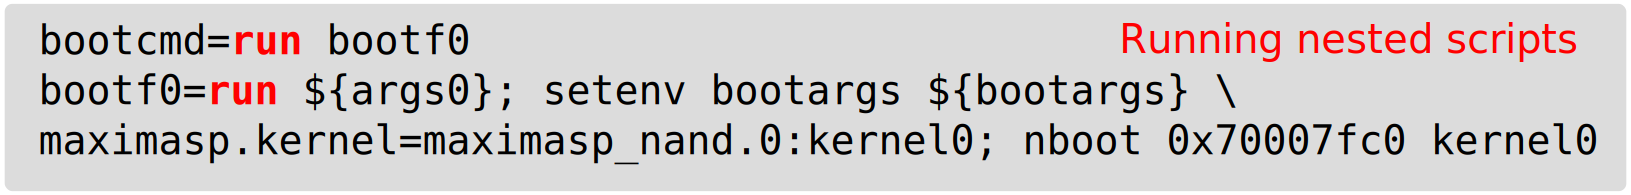
\includegraphics[width=\textwidth]{slides/boot-time-bootloader/u-boot-bad-scripts.pdf}
\end{center}
Let's replace this by:
\begin{block}{}
\footnotesize
\begin{verbatim}
setenv bootargs 'mem=128M console=tty0 consoleblank=0
console=ttyS0,57600 \
mtdparts=maximasp_nand.0:2M(u-boot)ro,512k(env0)ro,512k(env1)ro,\
4M(kernel0),4M(kernel1),5M(kernel2),100M(root0),100M(root1),-(other)\
rw ubi.mtd=root0 root=ubi0:rootfs rootfstype=ubifs earlyprintk debug \
user_debug=28 maximasp.board=EEKv1.3.x \
maximasp.kernel=maximasp_nand.0:kernel0'
setenv bootcmd 'nboot 0x70007fc0 kernel0'
\end{verbatim}
\end{block}
This saved 56 ms on this ARM9 system (400 MHz)!
\end{frame}

\begin{frame}
\frametitle{Bootloader: copy the exact kernel size}
\begin{itemize}
\item When copying the kernel from {\bf raw} flash or MMC to RAM, we still see
      many systems that copy too many bytes, not taking the
      exact kernel size into account.
\item A solution is to store the exact size of the kernel in an environment
      variable, and use it a kernel loading time.
\item Of course, that's not needed when the kernel is loaded from a
      filesystem, which knows how big the file is.
\end{itemize}
\end{frame}
